\documentclass[10pt,a4paper]{article}

% --- Core Geometry and Page Setup ---
\usepackage[a4paper, left=1.2cm, right=1.2cm, top=1.1cm, bottom=1.1cm, footskip=14pt]{geometry}
\usepackage[utf8]{inputenc}
\usepackage[T1]{fontenc}
\usepackage{helvet}
\renewcommand{\familydefault}{\sfdefault}
\usepackage{microtype}
\usepackage{graphicx}
\usepackage{xcolor}
\usepackage{tcolorbox}
\tcbuselibrary{skins,raster}
\usepackage{tabularx}
\usepackage{booktabs}
\usepackage{colortbl}
\usepackage{enumitem}
\usepackage{amssymb}
\usepackage{tfrupee}
\usepackage{lastpage}
\usepackage{fancyhdr}

% --- High-Contrast Enterprise Color Palette ---
\definecolor{NavyDark}{HTML}{0B2545}
\definecolor{NavyPrimary}{HTML}{134074}
\definecolor{TealPrimary}{HTML}{0077B6}
\definecolor{CyanAccent}{HTML}{0096C7}
\definecolor{EmeraldGreen}{HTML}{059669}
\definecolor{EmeraldBg}{HTML}{ECFDF5}
\definecolor{EmeraldBorder}{HTML}{10B981}
\definecolor{AmberDark}{HTML}{B45309}
\definecolor{AmberBg}{HTML}{FFFBEB}
\definecolor{AmberBorder}{HTML}{F59E0B}
\definecolor{CardBg}{HTML}{FFFFFF}
\definecolor{PageBg}{HTML}{F8FAFC}
\definecolor{BorderLight}{HTML}{CBD5E1}
\definecolor{TextPrimary}{HTML}{0F172A}
\definecolor{TextSecondary}{HTML}{334155}
\definecolor{TextMuted}{HTML}{64748B}
\definecolor{TableStripe}{HTML}{F1F5F9}
\definecolor{HeroColumnBg}{HTML}{F0FDF4}
\definecolor{HeroColumnBorder}{HTML}{86EFAC}

% --- Running Headers and Footers ---
\pagestyle{fancy}
\fancyhf{}
\renewcommand{\headrulewidth}{0pt}
\fancyfoot[L]{\fontsize{7.5}{9}\selectfont \textcolor{TextMuted}{\textbf{Athena Engineering Corp} $\bullet$ Kakinada, Andhra Pradesh, India $\bullet$ \textbf{aquaCON\textsuperscript{\tiny TM}}}}
\fancyfoot[C]{\fontsize{7.5}{9}\selectfont \textcolor{TealPrimary}{\textbf{COMMERCIAL PRODUCT BRIEF $\vert$ FOR PROSPECTIVE CLIENTS}}}
\fancyfoot[R]{\fontsize{7.5}{9}\selectfont \textcolor{TextMuted}{\textbf{Page \thepage\ of \pageref{LastPage}}}}

\setlength{\parindent}{0pt}
\setlength{\parskip}{0pt}

\begin{document}

% ==============================================================================
% PAGE 1: EXECUTIVE BRIEF, PROBLEM/SOLUTION, HERO VISUAL & HARDWARE SPECS
% ==============================================================================

% --- Enterprise Header Banner with Official Athena Logo ---
\begin{tcolorbox}[
  enhanced,
  colback=NavyDark,
  colframe=NavyDark,
  colupper=white,
  arc=2.5mm,
  boxrule=0pt,
  left=14pt, right=14pt, top=8pt, bottom=8pt
]
  \begin{minipage}[c]{0.70\linewidth}
    {\fontsize{8}{10}\selectfont \textbf{\textcolor{CyanAccent}{COMMERCIAL SOLUTION BRIEF}} $\vert$ ADVANCED AQUACULTURE TECHNOLOGIES}\\[3pt]
    {\fontsize{18}{22}\selectfont \textbf{aquaCON\textsuperscript{\tiny TM} Intelligent Solar Feeder System}}\\[3pt]
    {\fontsize{9.5}{12}\selectfont \textcolor{BorderLight}{Autonomous Precision Dosing, Long-Range LoRaWAN\textsuperscript{\tiny \textregistered}\ Mesh \& Real-Time Cloud Intelligence}}
  \end{minipage}\hfill
  \begin{minipage}[c]{0.28\linewidth}
    \raggedleft
    \begin{tcolorbox}[
      enhanced,
      colback=white,
      colframe=white,
      arc=2mm,
      boxrule=0pt,
      halign=center,
      valign=center,
      top=3pt, bottom=3pt, left=6pt, right=6pt
    ]
      
\includegraphics[height=1.25cm, keepaspectratio=true]{athena_logo.png}
    \end{tcolorbox}
  \end{minipage}
\end{tcolorbox}

\vspace{5pt}

% --- Executive KPI Highlight Ribbon (5 Uniform Strategic Metrics) ---
\begin{tcolorbox}[
  enhanced,
  colback=PageBg,
  colframe=BorderLight,
  arc=2mm,
  boxrule=0.8pt,
  left=4pt, right=4pt, top=7pt, bottom=7pt
]
  \begin{minipage}[t]{0.19\linewidth}
    \centering
    {\fontsize{14}{16}\selectfont \textbf{\textcolor{EmeraldGreen}{15\% -- 22\%}}}\\[2pt]
    {\fontsize{7.5}{9}\selectfont \textbf{FCR Improvement}\\(Saves 8--10 Tons Feed)}
  \end{minipage}\hfill
  \begin{minipage}[t]{0.19\linewidth}
    \centering
    {\fontsize{14}{16}\selectfont \textbf{\textcolor{TealPrimary}{100\% Solar}}}\\[2pt]
    {\fontsize{7.5}{9}\selectfont \textbf{Zero Shore Cabling}\\(LiFePO4 Powerplant)}
  \end{minipage}\hfill
  \begin{minipage}[t]{0.19\linewidth}
    \centering
    {\fontsize{14}{16}\selectfont \textbf{\textcolor{NavyPrimary}{15 km Range}}}\\[2pt]
    {\fontsize{7.5}{9}\selectfont \textbf{LoRaWAN\textsuperscript{\tiny \textregistered}\ Telemetry}\\(Farm-Wide Coverage)}
  \end{minipage}\hfill
  \begin{minipage}[t]{0.19\linewidth}
    \centering
    {\fontsize{14}{16}\selectfont \textbf{\textcolor{EmeraldGreen}{\rupee 0 / Feeder}}}\\[2pt]
    {\fontsize{7.5}{9}\selectfont \textbf{Zero Feeder SIMs}\\(1 Central Gateway)}
  \end{minipage}\hfill
  \begin{minipage}[t]{0.19\linewidth}
    \centering
    {\fontsize{14}{16}\selectfont \textbf{\textcolor{AmberDark}{$<$ 1 Crop}}}\\[2pt]
    {\fontsize{7.5}{9}\selectfont \textbf{Full Payback}\\(ROI in 90--120 Days)}
  \end{minipage}
\end{tcolorbox}

\vspace{6pt}

% --- The Problem vs The Solution (Two Balanced Cards with Maximum Contrast) ---
\begin{minipage}[t]{0.488\linewidth}
  \begin{tcolorbox}[
    enhanced,
    colback=CardBg,
    colframe=AmberBorder,
    arc=2mm,
    boxrule=1.1pt,
    title={\fontsize{8.5}{10.5}\selectfont \textbf{\textcolor{white}{The Industry Challenge: Costly Feeding Inefficiency}}},
    coltitle=white,
    colbacktitle=AmberDark,
    top=7pt, bottom=7pt, left=8pt, right=8pt
  ]
    {\fontsize{7.8}{10.4}\selectfont \textcolor{TextPrimary}{
    Feed accounts for \textbf{50\% to 70\% of total operational expenditure} in commercial aquaculture. Traditional manual hand-feeding and dumb timer dispensers suffer from crippling flaws:
    \begin{itemize}[leftmargin=11pt, itemsep=2.5pt, topsep=3pt, parsep=0pt]
      \item \textbf{Feed Wastage \& High FCR:} Hand-broadcast feeding is irregular. Uneaten feed accumulates on pond bottoms, rotting into toxic ammonia spikes and causing severe shrimp mortality.
      \item \textbf{Blind Conventional Dispensers:} Mechanical timers dump feed blindly during hopper jams or empty feed situations, burning out motors and leaving shrimp starved.
      \item \textbf{Dangerous Underwater Cabling:} Running 230V AC shore power across saline water creates severe electrocution hazards, frequent tripping, and expensive pond trenching.
      \item \textbf{High Recurring Telecom Costs:} Installing individual cellular SIM cards on 50+ feeders wastes over \textbf{\rupee 2,00,000+ per year} in recurring monthly data bills.
    \end{itemize}
    }}
  \end{tcolorbox}
\end{minipage}
\hfill
\begin{minipage}[t]{0.488\linewidth}
  \begin{tcolorbox}[
    enhanced,
    colback=CardBg,
    colframe=TealPrimary,
    arc=2mm,
    boxrule=1.1pt,
    title={\fontsize{8.5}{10.5}\selectfont \textbf{\textcolor{white}{The aquaCON\textsuperscript{\tiny TM} Solution: Autonomous Precision Dosing}}},
    coltitle=white,
    colbacktitle=TealPrimary,
    top=7pt, bottom=7pt, left=8pt, right=8pt
  ]
    {\fontsize{7.8}{10.4}\selectfont \textcolor{TextPrimary}{
    \textbf{aquaCON\textsuperscript{\tiny TM}} is an industrial-grade automated feeding system engineered specifically to slash Feed Conversion Ratio (FCR) and maximize farm profitability:
    \begin{itemize}[leftmargin=11pt, itemsep=2.5pt, topsep=3pt, parsep=0pt]
      \item \textbf{Dynamic Schedule Recalculation:} If a pause occurs or the hopper is refilled mid-day, the smart edge processor recalculates remaining intervals to dispense the exact target quota before dusk.
      \item \textbf{Optical \& Inductive Jam Interlocks:} Rotary stroke sensors verify full paddle discharge; automatic reverse-clearance pulses eliminate feed chute bridging.
      \item \textbf{Acoustic Parabolic Distribution:} High-velocity precision impeller broadcasts pellets smoothly in a calibrated 8--15\,m arc with zero crumble.
      \item \textbf{100\% Solar Power Autonomy:} Integrated 50W monocrystalline solar PV and automotive-grade LiFePO4 battery deliver 7+ days of sunless operation.
    \end{itemize}
    }}
  \end{tcolorbox}
\end{minipage}

\vspace{6pt}

% --- Hero Visual Showcase with Key Engineering Innovations ---
\begin{tcolorbox}[
  enhanced,
  colback=CardBg,
  colframe=BorderLight,
  arc=2mm,
  boxrule=0.8pt,
  top=6pt, bottom=6pt, left=8pt, right=8pt
]
  \begin{minipage}[c]{0.53\linewidth}
    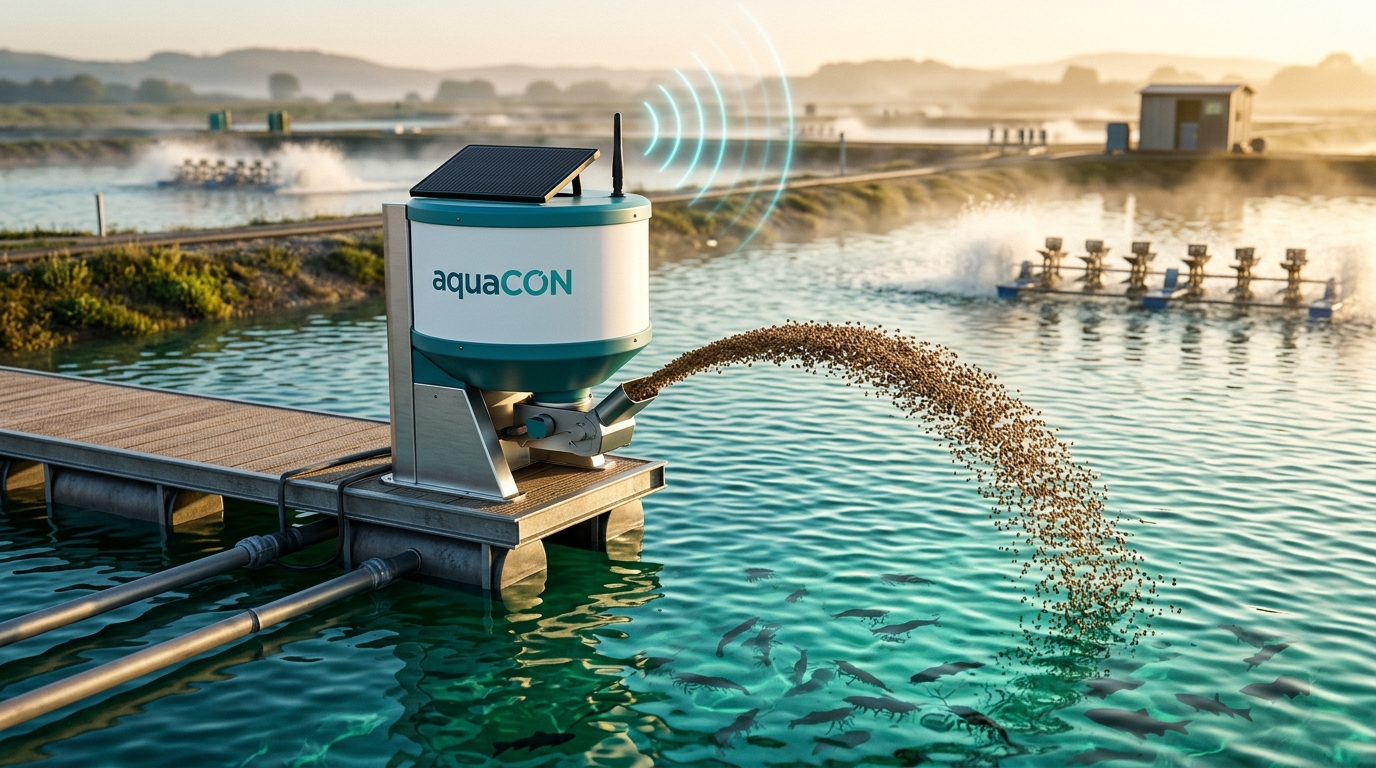
\includegraphics[width=\linewidth, height=5.1cm, keepaspectratio=false]{hero_feeder.jpg}
    \vspace{2pt}
    \centering
    {\fontsize{7}{8.5}\selectfont \textcolor{TextMuted}{\textbf{Figure 1:} aquaCON\textsuperscript{\tiny TM} Solar Smart Feeder broadcasting calibrated feed pellets across pond water surface at dawn with long-range LoRaWAN\textsuperscript{\tiny \textregistered}\ RF telemetry link.}}
  \end{minipage}\hfill
  \begin{minipage}[c]{0.44\linewidth}
    {\fontsize{8.5}{11}\selectfont \textbf{\textcolor{NavyDark}{Key Engineering Innovations:}}}\\[3pt]
    {\fontsize{7.5}{10}\selectfont \textcolor{TextPrimary}{
    \textbf{\textcolor{TealPrimary}{$\blacktriangleright$ Sub-Gram Dosing Precision:}}\\
    Calibrated micro-dosing (50\,g to 500\,g per burst) with $\pm$1.5\% repeatability ensures shrimp consume feed instantaneously without nutrient leaching.\\[3pt]
    \textbf{\textcolor{TealPrimary}{$\blacktriangleright$ Anti-Bridging Chute Geometry:}}\\
    Specialized low-friction hopper cone with integrated agitator prevents pellet compaction across all pellet sizes (0.8\,mm to 3.5\,mm).\\[3pt]
    \textbf{\textcolor{TealPrimary}{$\blacktriangleright$ Long-Range LoRaWAN\textsuperscript{\tiny \textregistered}\ Telemetry:}}\\
    Transmits dispensed kilograms, battery health, solar charging, and motor status up to 15\,km line-of-sight to the central farm gateway.\\[3pt]
    \textbf{\textcolor{TealPrimary}{$\blacktriangleright$ Heavy-Duty Marine Ingress Protection:}}\\
    UV-stabilized virgin polymer hopper and 316 stainless steel chassis engineered for corrosive coastal saline environments.
    }}
  \end{minipage}
\end{tcolorbox}

\vspace{6pt}

% --- Feeder Hardware Specifications Table (Full Width, Uniform & Pristine) ---
{\fontsize{8.5}{10.5}\selectfont \textbf{\textcolor{NavyDark}{aquaCON\textsuperscript{\tiny TM} Feeder Node Hardware Specifications}}}
\vspace{2pt}

\begin{tcolorbox}[
  enhanced,
  colback=CardBg,
  colframe=NavyPrimary,
  arc=2mm,
  boxrule=0.9pt,
  left=0pt, right=0pt, top=0pt, bottom=0pt
]
  \fontsize{7.3}{9.2}\selectfont
  \begin{tabularx}{\linewidth}{@{}p{2.6cm} X p{2.6cm} X@{}}
    \rowcolor{TableStripe}
    \textbf{Hopper Capacity:} & 120\,kg / 250\,kg UV Virgin Polymer & \textbf{Dosing Precision:} & 50\,g -- 500\,g per burst ($\pm$1.5\%)\\
    \textbf{Spread Radius:} & 8 to 15 meters parabolic arc & \textbf{Supported Pellets:} & 0.8\,mm to 3.5\,mm floating / sinking\\
    \rowcolor{TableStripe}
    \textbf{Solar Power:} & 50W Monocrystalline PV Panel & \textbf{Battery System:} & 12.8V LiFePO4 Smart BMS (7+ days reserve)\\
    \textbf{In-Pond Wireless:} & LoRaWAN\textsuperscript{\tiny \textregistered}\ Sub-GHz (865--868 / 915--928) & \textbf{RF Range:} & Up to 15\,km to Central Farm Gateway\\
    \rowcolor{TableStripe}
    \textbf{Ingress Rating:} & IP67 Weatherproof \& Marine Grade & \textbf{Jam Protection:} & Inductive Rotary Sensor + Reverse Pulse\\
    \textbf{Operational Mode:} & Dynamic Schedule (06:00 to 18:00) & \textbf{Safety Interlocks:} & Motor Overcurrent, Empty Feed Detection\\
  \end{tabularx}
\end{tcolorbox}

\newpage

% ==============================================================================
% PAGE 2: ARCHITECTURE, COMPETITIVE MATRIX, ROI (INR) & CORPORATE PROFILE
% ==============================================================================

% --- Page 2 Top Header Banner ---
\begin{tcolorbox}[
  enhanced,
  colback=NavyPrimary,
  colframe=NavyPrimary,
  colupper=white,
  arc=2.5mm,
  boxrule=0pt,
  left=14pt, right=14pt, top=8pt, bottom=8pt
]
  \begin{minipage}[c]{0.70\linewidth}
    {\fontsize{13}{16}\selectfont \textbf{Enterprise Architecture \& Competitive Differentiation}}\\[2pt]
    {\fontsize{8.5}{11}\selectfont \textcolor{CyanAccent}{From Pond Edge to Executive Cloud: Complete Visibility, Zero SIM Overhead, Proven ROI}}
  \end{minipage}\hfill
  \begin{minipage}[c]{0.28\linewidth}
    \raggedleft
    {\fontsize{9.5}{11.5}\selectfont \textbf{aquaCON\textsuperscript{\tiny TM} Solution Brief}}\\[1pt]
    {\fontsize{7.5}{9}\selectfont \textcolor{BorderLight}{Architecture \& Financial Model}}
  \end{minipage}
\end{tcolorbox}

\vspace{5pt}

% --- Solution Architecture Visual & 3-Tier Enterprise Topology ---
\begin{tcolorbox}[
  enhanced,
  colback=CardBg,
  colframe=BorderLight,
  arc=2mm,
  boxrule=0.8pt,
  top=6pt, bottom=6pt, left=8pt, right=8pt
]
  \begin{minipage}[c]{0.45\linewidth}
    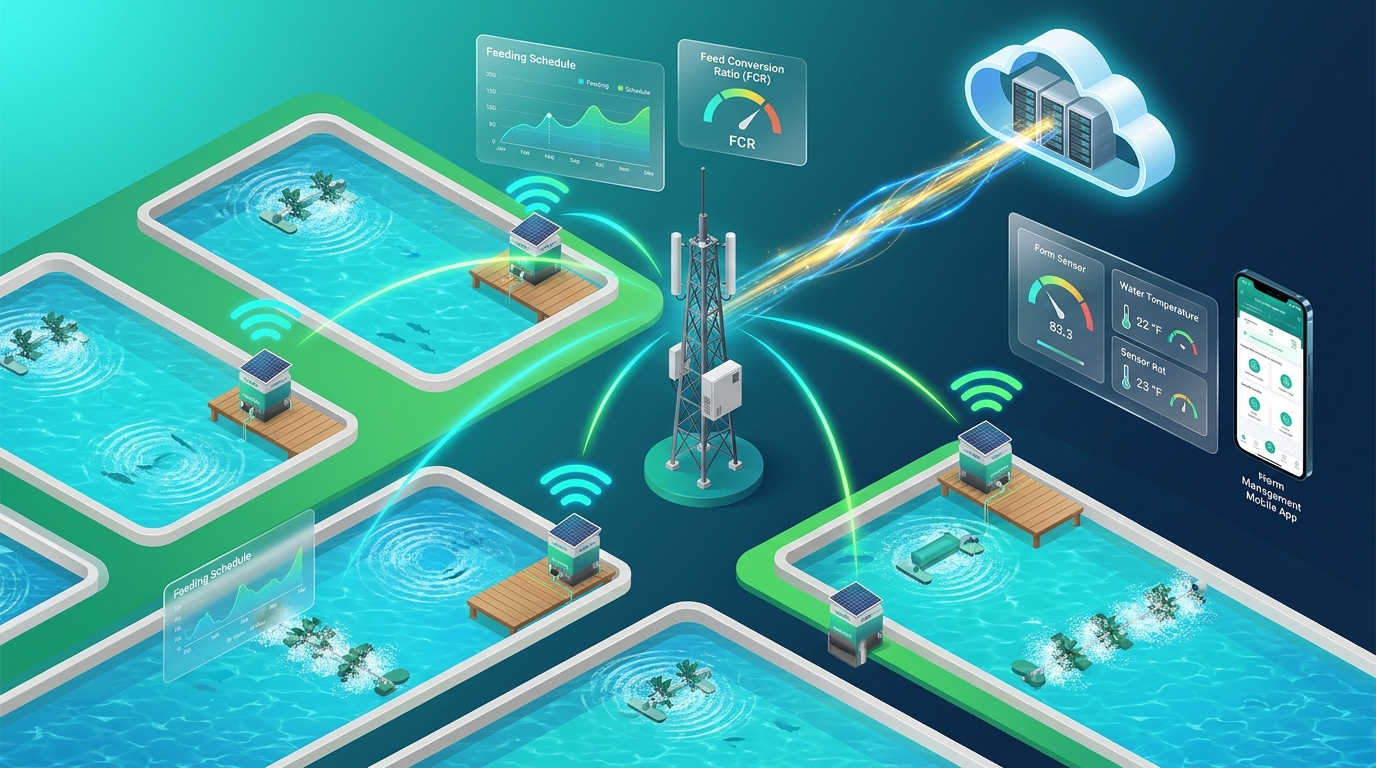
\includegraphics[width=\linewidth, height=4.5cm, keepaspectratio=false]{solution_architecture.jpg}
  \end{minipage}\hfill
  \begin{minipage}[c]{0.52\linewidth}
    {\fontsize{8.5}{11}\selectfont \textbf{\textcolor{NavyDark}{3-Tier Scalable IoT Farm Ecosystem:}}}\\[2pt]
    {\fontsize{7.5}{9.8}\selectfont \textcolor{TextPrimary}{
    \textbf{\textcolor{TealPrimary}{Tier 1: Intelligent Feeder Nodes (Pond-Side):}}\\
    Autonomous solar feeders located on pond piers or floating frames. Each node continuously monitors battery status, solar harvesting, motor drive current, and dispense cycle completions, broadcasting lightweight telemetry packets over LoRaWAN\textsuperscript{\tiny \textregistered}.\\[3pt]
    \textbf{\textcolor{TealPrimary}{Tier 2: Central Industrial Gateway (Farm Mast):}}\\
    A single high-gain industrial gateway mounted on a central mast covers \textbf{50 to 200+ ponds across a 15\,km radius}. Aggregates all pond uplinks and bridges to the cloud via \textbf{tri-redundant Wi-Fi, Industrial Ethernet, or 4G LTE cellular}. Eliminates per-feeder cellular SIM costs.\\[3pt]
    \textbf{\textcolor{TealPrimary}{Tier 3: aquaCON\textsuperscript{\tiny TM} Cloud Intelligence Platform:}}\\
    Enterprise cloud infrastructure provides real-time supervisor dashboards, automatic daily schedule calculation, historical event auditing, and instant SMS/call alerts for hopper empty or jam events.
    }}
  \end{minipage}
\end{tcolorbox}

\vspace{6pt}

% --- Redesigned High-Impact Competitive Differentiation Matrix ---
{\fontsize{8.5}{10.5}\selectfont \textbf{\textcolor{NavyDark}{Competitive Differentiation Matrix: Why aquaCON\textsuperscript{\tiny TM} Outperforms}}}
\vspace{2pt}

\begin{tcolorbox}[
  enhanced,
  colback=CardBg,
  colframe=NavyDark,
  arc=2mm,
  boxrule=1pt,
  left=0pt, right=0pt, top=0pt, bottom=0pt
]
  \renewcommand{\arraystretch}{1.3}
  \fontsize{7.2}{9.0}\selectfont
  \begin{tabularx}{\linewidth}{@{}p{3.8cm} >{\centering\arraybackslash}p{4.0cm} >{\centering\arraybackslash}p{4.2cm} >{\centering\arraybackslash}X@{}}
    \rowcolor{NavyDark}
    \textcolor{white}{\textbf{Core Capability}} &
    \textcolor{white}{\textbf{Manual Hand Feeding}} &
    \textcolor{white}{\textbf{Traditional Timer Feeders}} &
    \textcolor{white}{\textbf{aquaCON\textsuperscript{\tiny TM} Smart Feeder}} \\

    \textbf{Feed Conversion Ratio (FCR)} &
    1.65 -- 1.85 (High Feed Waste) &
    1.45 -- 1.60 (Blind Fixed Cycles) &
    \cellcolor{HeroColumnBg}\textbf{\textcolor{EmeraldGreen}{\checkmark\ 1.20 -- 1.30 (15\%--22\% Saved)}} \\
    \rowcolor{TableStripe}
    \textbf{Labor Deployment} &
    4 -- 6 Field Workers per 10 Ponds &
    2 Workers (Frequent manual checks) &
    \cellcolor{HeroColumnBg}\textbf{\textcolor{EmeraldGreen}{\checkmark\ 1 Supervisor manages 50+ Ponds}} \\

    \textbf{Power Infrastructure} &
    Manual labor dependent &
    Dangerous 230V Shore Cables in Water &
    \cellcolor{HeroColumnBg}\textbf{\textcolor{TealPrimary}{\checkmark\ 100\% Solar + LiFePO4 (Zero Cables)}} \\
    \rowcolor{TableStripe}
    \textbf{Farm Wireless Connectivity} &
    None (Vulnerable paper logs) &
    None / Short-Range Bluetooth ($<$15\,m) &
    \cellcolor{HeroColumnBg}\textbf{\textcolor{NavyPrimary}{\checkmark\ Long-Range LoRaWAN\textsuperscript{\tiny \textregistered}\ (15\,km)}} \\

    \textbf{Annual SIM Card Cost} &
    \rupee 0 (No connectivity) &
    \rupee 3,500 -- \rupee 5,000 / feeder / year &
    \cellcolor{HeroColumnBg}\textbf{\textcolor{EmeraldGreen}{\checkmark\ \rupee 0 Per Feeder (1 Central Gateway)}} \\
    \rowcolor{TableStripe}
    \textbf{Jam \& Empty Interlock} &
    Discovered hours later (Starvation) &
    None (Burned motors, wasted schedule) &
    \cellcolor{HeroColumnBg}\textbf{\textcolor{EmeraldGreen}{\checkmark\ Real-Time Sensor Interlock \& Alert}} \\

    \textbf{Dynamic Schedule Recalc} &
    None (Manual human guesswork) &
    Impossible on mechanical timers &
    \cellcolor{HeroColumnBg}\textbf{\textcolor{TealPrimary}{\checkmark\ Autonomous Mid-Day Recalculation}} \\
    \rowcolor{TableStripe}
    \textbf{Audit Trail \& Cloud App} &
    None &
    None &
    \cellcolor{HeroColumnBg}\textbf{\textcolor{NavyDark}{\checkmark\ Real-Time Cloud App \& Event History}} \\
  \end{tabularx}
\end{tcolorbox}

\vspace{6pt}

% --- Bottom Row: Financial Impact in Indian Rupees (INR) vs Authentic Corporate Contact ---
\begin{minipage}[t]{0.488\linewidth}
  \begin{tcolorbox}[
    enhanced,
    colback=EmeraldBg,
    colframe=EmeraldBorder,
    arc=2mm,
    boxrule=1.1pt,
    title={\fontsize{8.5}{10.5}\selectfont \textbf{\textcolor{white}{Customer ROI Model: 10-Hectare Farm (Indian Rupees)}}},
    coltitle=white,
    colbacktitle=EmeraldGreen,
    top=7pt, bottom=7pt, left=8pt, right=8pt
  ]
    {\fontsize{7.4}{9.6}\selectfont \textcolor{TextPrimary}{
    \textbf{Commercial baseline: 10 ponds consuming 40,000\,kg feed per crop:}
    \begin{itemize}[leftmargin=10pt, itemsep=2.5pt, topsep=2pt, parsep=0pt]
      \item \textbf{Feed Cost Savings:} Reducing FCR from 1.60 to 1.30 saves \textbf{7,500\,kg of commercial feed} per harvest. At \rupee 100/kg, this delivers \textbf{\rupee 7,50,000 to \rupee 10,00,000 direct cash savings per crop}.
      \item \textbf{Labor Payroll Savings:} Reduces feeding labor from 4 workers to 1 supervisor, saving \textbf{\rupee 1,80,000 to \rupee 2,40,000 per crop cycle}.
      \item \textbf{Telecom SIM Savings:} Eliminates \rupee 2,00,000+ per year in wasted cellular data fees across farm feeders.
      \item \textbf{Rapid Capital Payback:} \textbf{Complete investment recovered in under 90 to 120 days (Within 1 crop cycle)}.
    \end{itemize}
    }}
  \end{tcolorbox}
\end{minipage}
\hfill
\begin{minipage}[t]{0.488\linewidth}
  \begin{tcolorbox}[
    enhanced,
    colback=CardBg,
    colframe=NavyDark,
    arc=2mm,
    boxrule=1.1pt,
    title={\fontsize{8.5}{10.5}\selectfont \textbf{\textcolor{white}{Athena Engineering Corp $\vert$ Kakinada, India}}},
    coltitle=white,
    colbacktitle=NavyDark,
    top=7pt, bottom=7pt, left=8pt, right=8pt
  ]
    {\fontsize{7.4}{9.6}\selectfont \textcolor{TextPrimary}{
    \textbf{Turnkey Farm Deployments \& Direct Support:}
    \begin{itemize}[leftmargin=10pt, itemsep=2pt, topsep=2pt, parsep=0pt]
      \item \textbf{On-Farm Pilot Deployments:} Turnkey installation of solar feeders and central gateway with on-site technician calibration.
      \item \textbf{Multi-Species Precision:} Calibrated for Vannamei shrimp, Black Tiger shrimp, Tilapia, and high-density marine cages.
      \item \textbf{Enterprise SLA \& Warranty:} 3-year hardware warranty with local engineering support from Kakinada.
    \end{itemize}
    \vspace{4pt}
    \begin{tcolorbox}[
      enhanced,
      colback=NavyDark,
      colframe=CyanAccent,
      colupper=white,
      arc=1.5mm,
      boxrule=0.8pt,
      top=4pt, bottom=4pt, left=6pt, right=6pt
    ]
      \centering
      {\fontsize{8.5}{10.5}\selectfont \textbf{\textcolor{white}{Schedule an On-Farm Demonstration \& Site Survey}}}\\[2pt]
      {\fontsize{7.5}{9}\selectfont \textcolor{CyanAccent}{\textbf{Athena Engineering Corp}} $\vert$ Kakinada, Andhra Pradesh, India}\\[1pt]
      {\fontsize{7}{8.5}\selectfont \textcolor{BorderLight}{Address: \textbf{2-48-22, 1st Street, 100 Buildings, Kakinada - 533003, AP}}}\\[1pt]
      {\fontsize{7}{8.5}\selectfont \textcolor{BorderLight}{Direct Commercial Lead: \textbf{+91 91546 96777} $\vert$ rc@athenaenggcorp.com}}\\[1pt]
      {\fontsize{7}{8.5}\selectfont \textcolor{BorderLight}{Official Website: \textbf{www.athenaenggcorp.com}}}
    \end{tcolorbox}
    }}
  \end{tcolorbox}
\end{minipage}

\end{document}
